\documentclass[11pt]{report} 

\usepackage{projectreport}

% ------------------------------------------------------------------------------
%  Title page 
% ------------------------------------------------------------------------------
\newcommand{\name}{Abhijith A., S. Praneel, Rashmi P., Arijit C., Goverdhan R. G. and Shridurga M.}
\newcommand{\course}{Interim Report}
\newcommand{\projecttitle}{Pneumonia Detection Challenge}
\newcommand{\submissiondate}{July 7 2024}


% ------------------------------------------------------------------------------
% Document
% ------------------------------------------------------------------------------
\begin{document}

\maketitle

% ------------------------------------------------------------------------------
% Top matter
% ------------------------------------------------------------------------------
\chapter*{Abstract}

This report presents a comprehensive exploration of pneumonia detection using computer vision techniques on chest radiographs. The study begins with an extensive Exploratory Data Analysis (EDA) to understand the dataset's structure and underlying patterns, including patient demographics and distribution of class labels. EDA findings revealed a balanced distribution of images across various patient ages, sexes, and view positions, although further data augmentation is suggested to enhance the dataset's diversity.

Subsequently, multiple convolutional neural network (CNN) models were developed and evaluated to classify images based on the presence of lung opacity. Model 1, using RMSprop optimizer, showed moderate performance but indicated potential overfitting. Model 2, utilizing the Adam optimizer, improved initial training stability but faced similar overfitting challenges. Model 3, a simplified architecture, demonstrated better training and validation accuracy after implementing improvement strategies like learning rate reduction and model checkpointing. Despite these efforts, the results highlighted the necessity for further tuning and advanced techniques to achieve optimal performance.

The project transitions into predicting the target variable, with plans to employ Region-based Convolutional Neural Networks (RCNN) in subsequent phases to enhance class label classification. Final model evaluation through confusion matrix and ROC curve analyses underscored the need for balancing sensitivity and specificity, with current metrics indicating areas for improvement.

Future steps involve comprehensive data augmentation, exploration of advanced architectures, and the incorporation of transfer learning to improve model performance. The findings and methodologies outlined in this report lay a solid foundation for continued advancements in automated pneumonia detection, aiming towards more accurate and reliable diagnostic tools in medical imaging.

\vspace{2cm}

\chapter*{Acknowledgements}
We extend our heartfelt gratitude to our mentor, Jayant, for his invaluable guidance throughout this project. His insights and expertise have been instrumental in shaping our work. We also express our sincere thanks to our program manager, Avaneesh, for his constant support and encouragement, which have motivated us to strive for excellence.

We are grateful to Great Learning for facilitating this learning platform and providing us with the necessary resources and tools. Their commitment to education and continuous support have significantly contributed to the success of our project.

\tableofcontents
\listoffigures
\listoftables

% ------------------------------------------------------------------------------
% Main matter
% ------------------------------------------------------------------------------
\newpage
\setcounter{page}{0}
\pagenumbering{arabic}
% ------------------------------------------------------------------------------
% Chapter 1
% ------------------------------------------------------------------------------
\chapter{Summary of Problem Statement, Data, and Findings}
\label{cha:chapter 1}


\section{Problem Statement}
\label{sec:chap1 section 1}

\subsection{Context}
\label{subsec:chap1 section 1.1}
Pneumonia is a significant health concern, responsible for over 15\% of deaths in children under 5 years old globally. In 2015, it caused 920,000 deaths among children under 5 worldwide and over 50,000 deaths in the United States. Diagnosing pneumonia accurately requires a detailed review of chest radiographs (CXR) by highly trained specialists, coupled with clinical history, vital signs, and laboratory tests. Pneumonia typically appears as increased opacity on CXRs, but other conditions, such as pulmonary edema, lung cancer, and pleural effusion, can complicate the diagnosis.

Given the volume of images that clinicians must review, there is a pressing need for automated tools to assist in diagnosing pneumonia efficiently.

\subsection{Project Objective}
\label{subsec:chap1 section 1.2}

Design a deep learning-based algorithm to detect pneumonia in medical images. Specifically, the algorithm should automatically locate lung opacities on chest radiographs.

\subsection{Project Background}
\label{subsec:chap1 section 1.3}
This problem is derived from the RSNA Pneumonia Detection Challenge on Kaggle, which aims to improve the efficiency and reach of diagnostic services using machine learning. The Radiological Society of North America (RSNA) has collaborated with the US National Institutes of Health, The Society of Thoracic Radiology, and MD.ai to create a rich dataset for this challenge. The goal is to automate the initial detection of potential pneumonia cases to prioritize and expedite their review. The original sources of data is cited: ~\cite{rui2015emergency, cdc2015deaths, franquet2018pneumonia, kelly2012chest, wang2017chestxray8}

\subsection{Importance}
\label{subsec:chap1 section 1.4}
Automating pneumonia detection can save lives by enabling quicker diagnosis and treatment, particularly in resource-limited settings.
\section{Data Description}
\label{sec:chap1 section 2}

\subsection{Dataset Overview:}
\label{subsec:chap1 section 2.1}

The provided dataset includes medical images stored in DICOM files (*.dcm). DICOM (Digital Imaging and Communications in Medicine) is a standard format for storing medical imaging information. Each DICOM file contains metadata about the image, such as patient information, image acquisition parameters, and annotations, as well as the underlying raw image data.

\subsection{Image Labels:}
\label{subsec:chap1 section 2.2}
The dataset includes images labeled as "Not Normal No Lung Opacity," indicating that while pneumonia was not detected, other abnormalities are present. These cases can mimic the appearance of pneumonia, adding complexity to the detection task.

\subsection{Source and Accessibility:}
\label{subsec:chap1 section 2.3}
The dataset is provided by the National Institutes of Health Clinical Center and is publicly available for research purposes. This rich dataset has been curated to aid in developing and validating machine learning algorithms for pneumonia detection.

\subsection{Data Characteristics:}
\label{subsec:chap1 section 2.4}
The images in the dataset vary in terms of quality, patient positioning, and other factors, which can affect the appearance of the chest radiographs and complicate the interpretation. This diversity in the dataset helps in training robust models that can generalize well across different clinical scenarios.

\section{Initial Findings}
\label{sec:chap1 section 3}

\subsection{Image Modality and Area:}
\label{subsec:chap1 section 3.1}

\begin{itemize}
	\item \textbf{Modality:} The images obtained are of type CR (Computed Radiography).
	\item \textbf{Area:} The images focus on the chest area.
\end{itemize}

\subsection{Dataset Characteristics:}
\label{subsec:chap1 section 3.2}

\begin{itemize}
	\item \textbf{Class Distribution:} The dataset presents a challenge due to the class distribution, with approximately 39\% of the data labeled as “No Lung Opacity/Not Normal.” This class may interfere with the model's ability to accurately detect pneumonia.
	\item \textbf{Class Imbalance:} The dataset is slightly imbalanced, which may affect the performance of the model.
\end{itemize}

\subsection{Patient and Bounding Box Details:}
\label{subsec:chap1 section 3.3}

\begin{itemize}
	\item \textbf{Unique Patient IDs:} There are 26,684 unique patient IDs in the dataset.
	\item \textbf{Bounding Boxes:}
	      \begin{itemize}
		      \item A total of 30,227 bounding boxes are present, as some patients have multiple bounding boxes.
		      \item Bounding boxes with coordinates ("x", "y", "width", "height") are null when the target is 0, indicating the absence of pneumonia.
		      \item Bounding boxes with non-null coordinates indicate the presence of pneumonia (Target is 1).
		      \item Of the 30,227 bounding boxes, 20,672 have Target 0, and 9,555 have Target 1.
	      \end{itemize}
\end{itemize}

\subsection{Distribution of Bounding Boxes:}
\label{subsec:chap1 section 3.4}

\begin{itemize}
	\item  Patients with no bounding box, single bounding box, and multiple bounding boxes are present.
	\item Among the 26,684 unique patient IDs:
	      \begin{itemize}
		      \item 87.27\% of patients have one bounding box.
		      \item 12.24\% of patients have two bounding boxes.
		      \item Patients with three bounding boxes account for 0.45\%.
		      \item Patients with four bounding boxes account for 0.05\%.
	      \end{itemize}
\end{itemize}

The initial findings highlight the key characteristics and challenges of the dataset, including the class imbalance and the distribution of bounding boxes, which will be crucial in developing and training an effective deep-learning model for pneumonia detection.

\section{Conclusion}
\label{sec:chap1 section 4}

In this chapter, we introduced the critical problem of pneumonia detection using deep learning algorithms applied to medical imaging. Pneumonia remains a significant health threat, especially among children under the age of five, and accurate and timely diagnosis is essential to saving lives. Traditional diagnostic methods rely on expert interpretation of chest radiographs (CXR), which can be challenging due to the presence of other conditions that mimic pneumonia.

We outlined the project's objective: to design an algorithm that can automatically detect lung opacities in chest radiographs, thereby aiding in the early and accurate diagnosis of pneumonia. The dataset provided for this task comprises DICOM images with associated metadata, presenting both opportunities and challenges. The presence of a significant proportion of images labeled as “No Lung Opacity/Not Normal” and the slight class imbalance pose specific difficulties for model training and accuracy.

Our initial findings highlighted the complexity of the dataset, with 39\% of the images belonging to the “No Lung Opacity/Not Normal” class and a noticeable class imbalance. The dataset contains 26,684 unique patient IDs and 30,227 bounding boxes, with a detailed analysis revealing varying numbers of bounding boxes per patient. This distribution further complicates the development of a robust detection algorithm.
% ------------------------------------------------------------------------------
% Chapter 2
% ------------------------------------------------------------------------------
\chapter{Another Chapter Heading} % enter the name of the chapter here
\label{cha:chapter 2 label} % enter the chapter label here (for cross referencing)

\blindtext[2]
% ------------------------------------------------------------------------------
% Chapter 3
% ------------------------------------------------------------------------------
\chapter{Deciding Models and Model Building}
\label{cha:chapter 3}

\section{Model Selection}
\label{sec:chap3 section 1}

\section{Model Building}
\label{sec:chap3 section 2}

% ------------------------------------------------------------------------------
% Chapter 4
% ------------------------------------------------------------------------------
\chapter{How to Improve Your Model Performance?}

\section{Improvement Strategies}
\label{sec:chap4 section 1}

After initial training, Model 3 showed promising results but still left room for improvement. To enhance the model's performance, several fine-tuning strategies were implemented. The ReduceLROnPlateau callback was used to monitor the validation accuracy, and the learning rate was reduced if the accuracy did not improve over ten epochs. This approach helped the model to converge more effectively by adjusting the learning rate dynamically. Additionally, ModelCheckpoint was utilized to save the best version of the model based on the minimum validation loss, ensuring that the most optimal weights were retained. Figure ~\ref{fig:cha-4 figure1} shows the training and validation accuracy and loss plots after implementing these strategies.

\begin{figure}
    \centering
    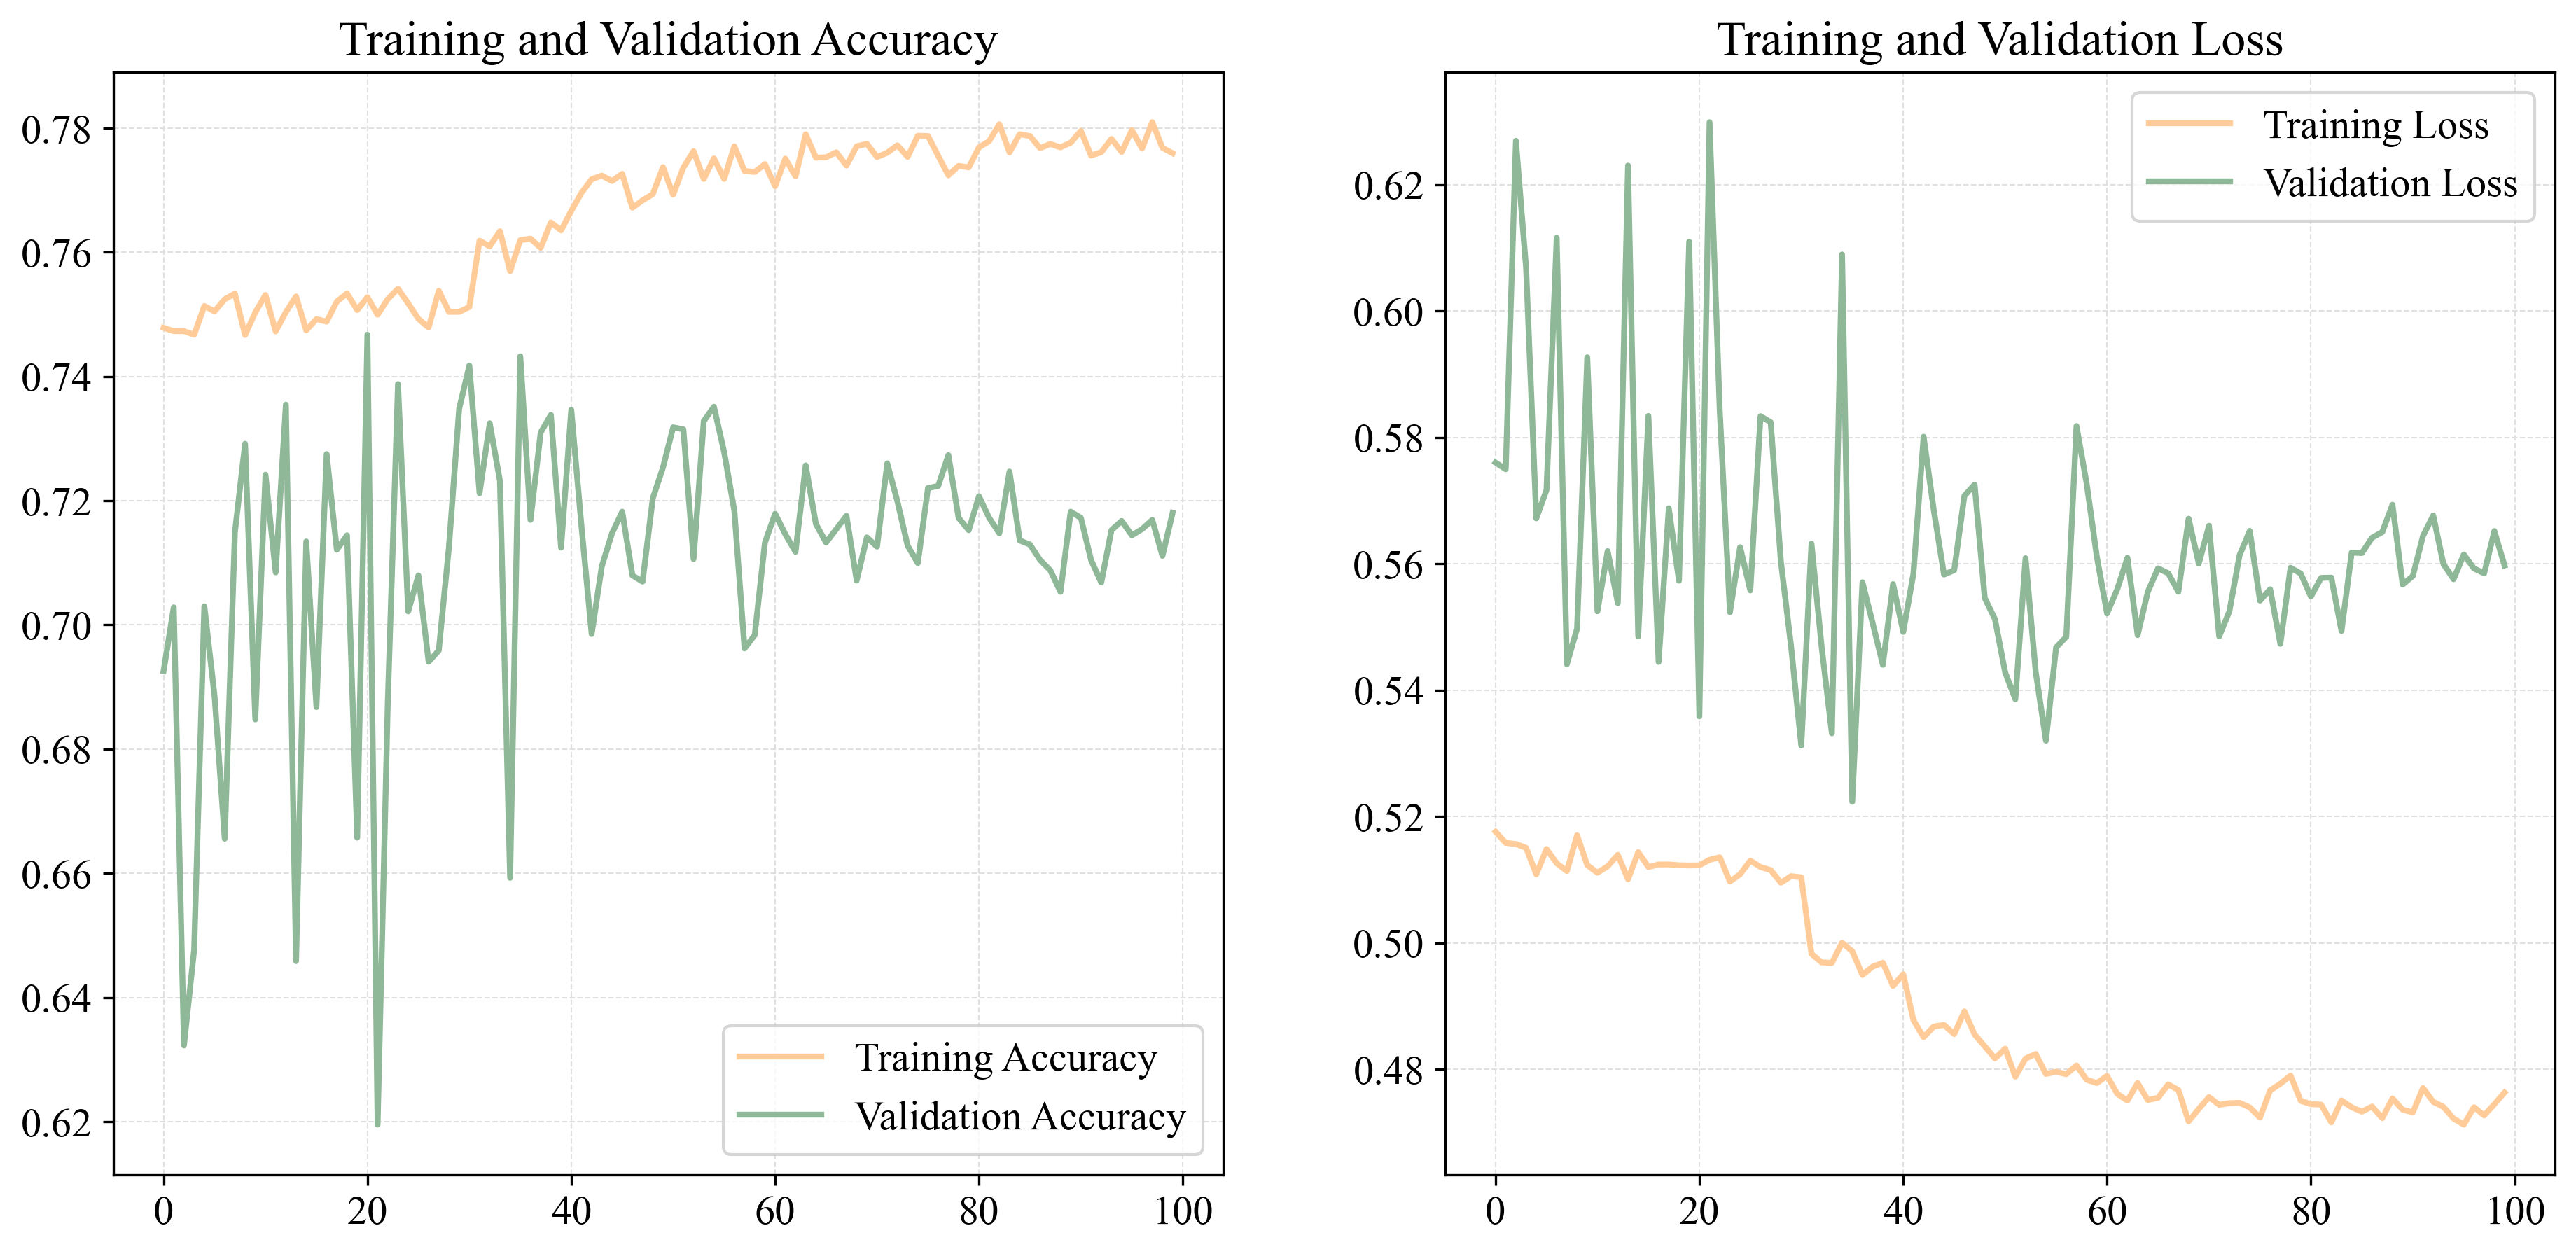
\includegraphics[width=0.8\textwidth]{figures/Figure32.png}
    \caption{Training and Validation Accuracy and Loss Plots}
    \label{fig:cha-4 figure1}
\end{figure}

These fine-tuning efforts led to noticeable improvements in both training and validation accuracy and loss. As depicted in the accompanying plots, the training accuracy steadily increased, and the validation accuracy showed a more stable trend compared to the initial runs. The training loss decreased significantly, and although the validation loss exhibited some fluctuations, the overall trend was positive, indicating a better generalization capability of the model.

\section {Model Evaluation}
\label{sec:chap4 section 2}
With the best model, we computed the confusion matrix and ROC curve. These are given in Figure ~\ref{fig:cha-4 figure2} and Figure ~\ref{fig:cha-4 figure3} respectively. The confusion matrix and ROC curve provide insights into the model's performance. The confusion matrix indicates that while the model correctly identifies a significant number of true positives (6154) and true negatives (12550), there is still a substantial number of false positives (3951) and false negatives (1492). This suggests that the model might benefit from further fine-tuning and potential adjustments in decision thresholds. The ROC curve, with an area under the curve (AUC) of 0.78, reflects a moderate level of discrimination between the positive and negative classes. While this is a promising start, aiming for a higher AUC by refining the model and its parameters will be crucial in improving overall accuracy and reliability.

\begin{figure}
    \centering
    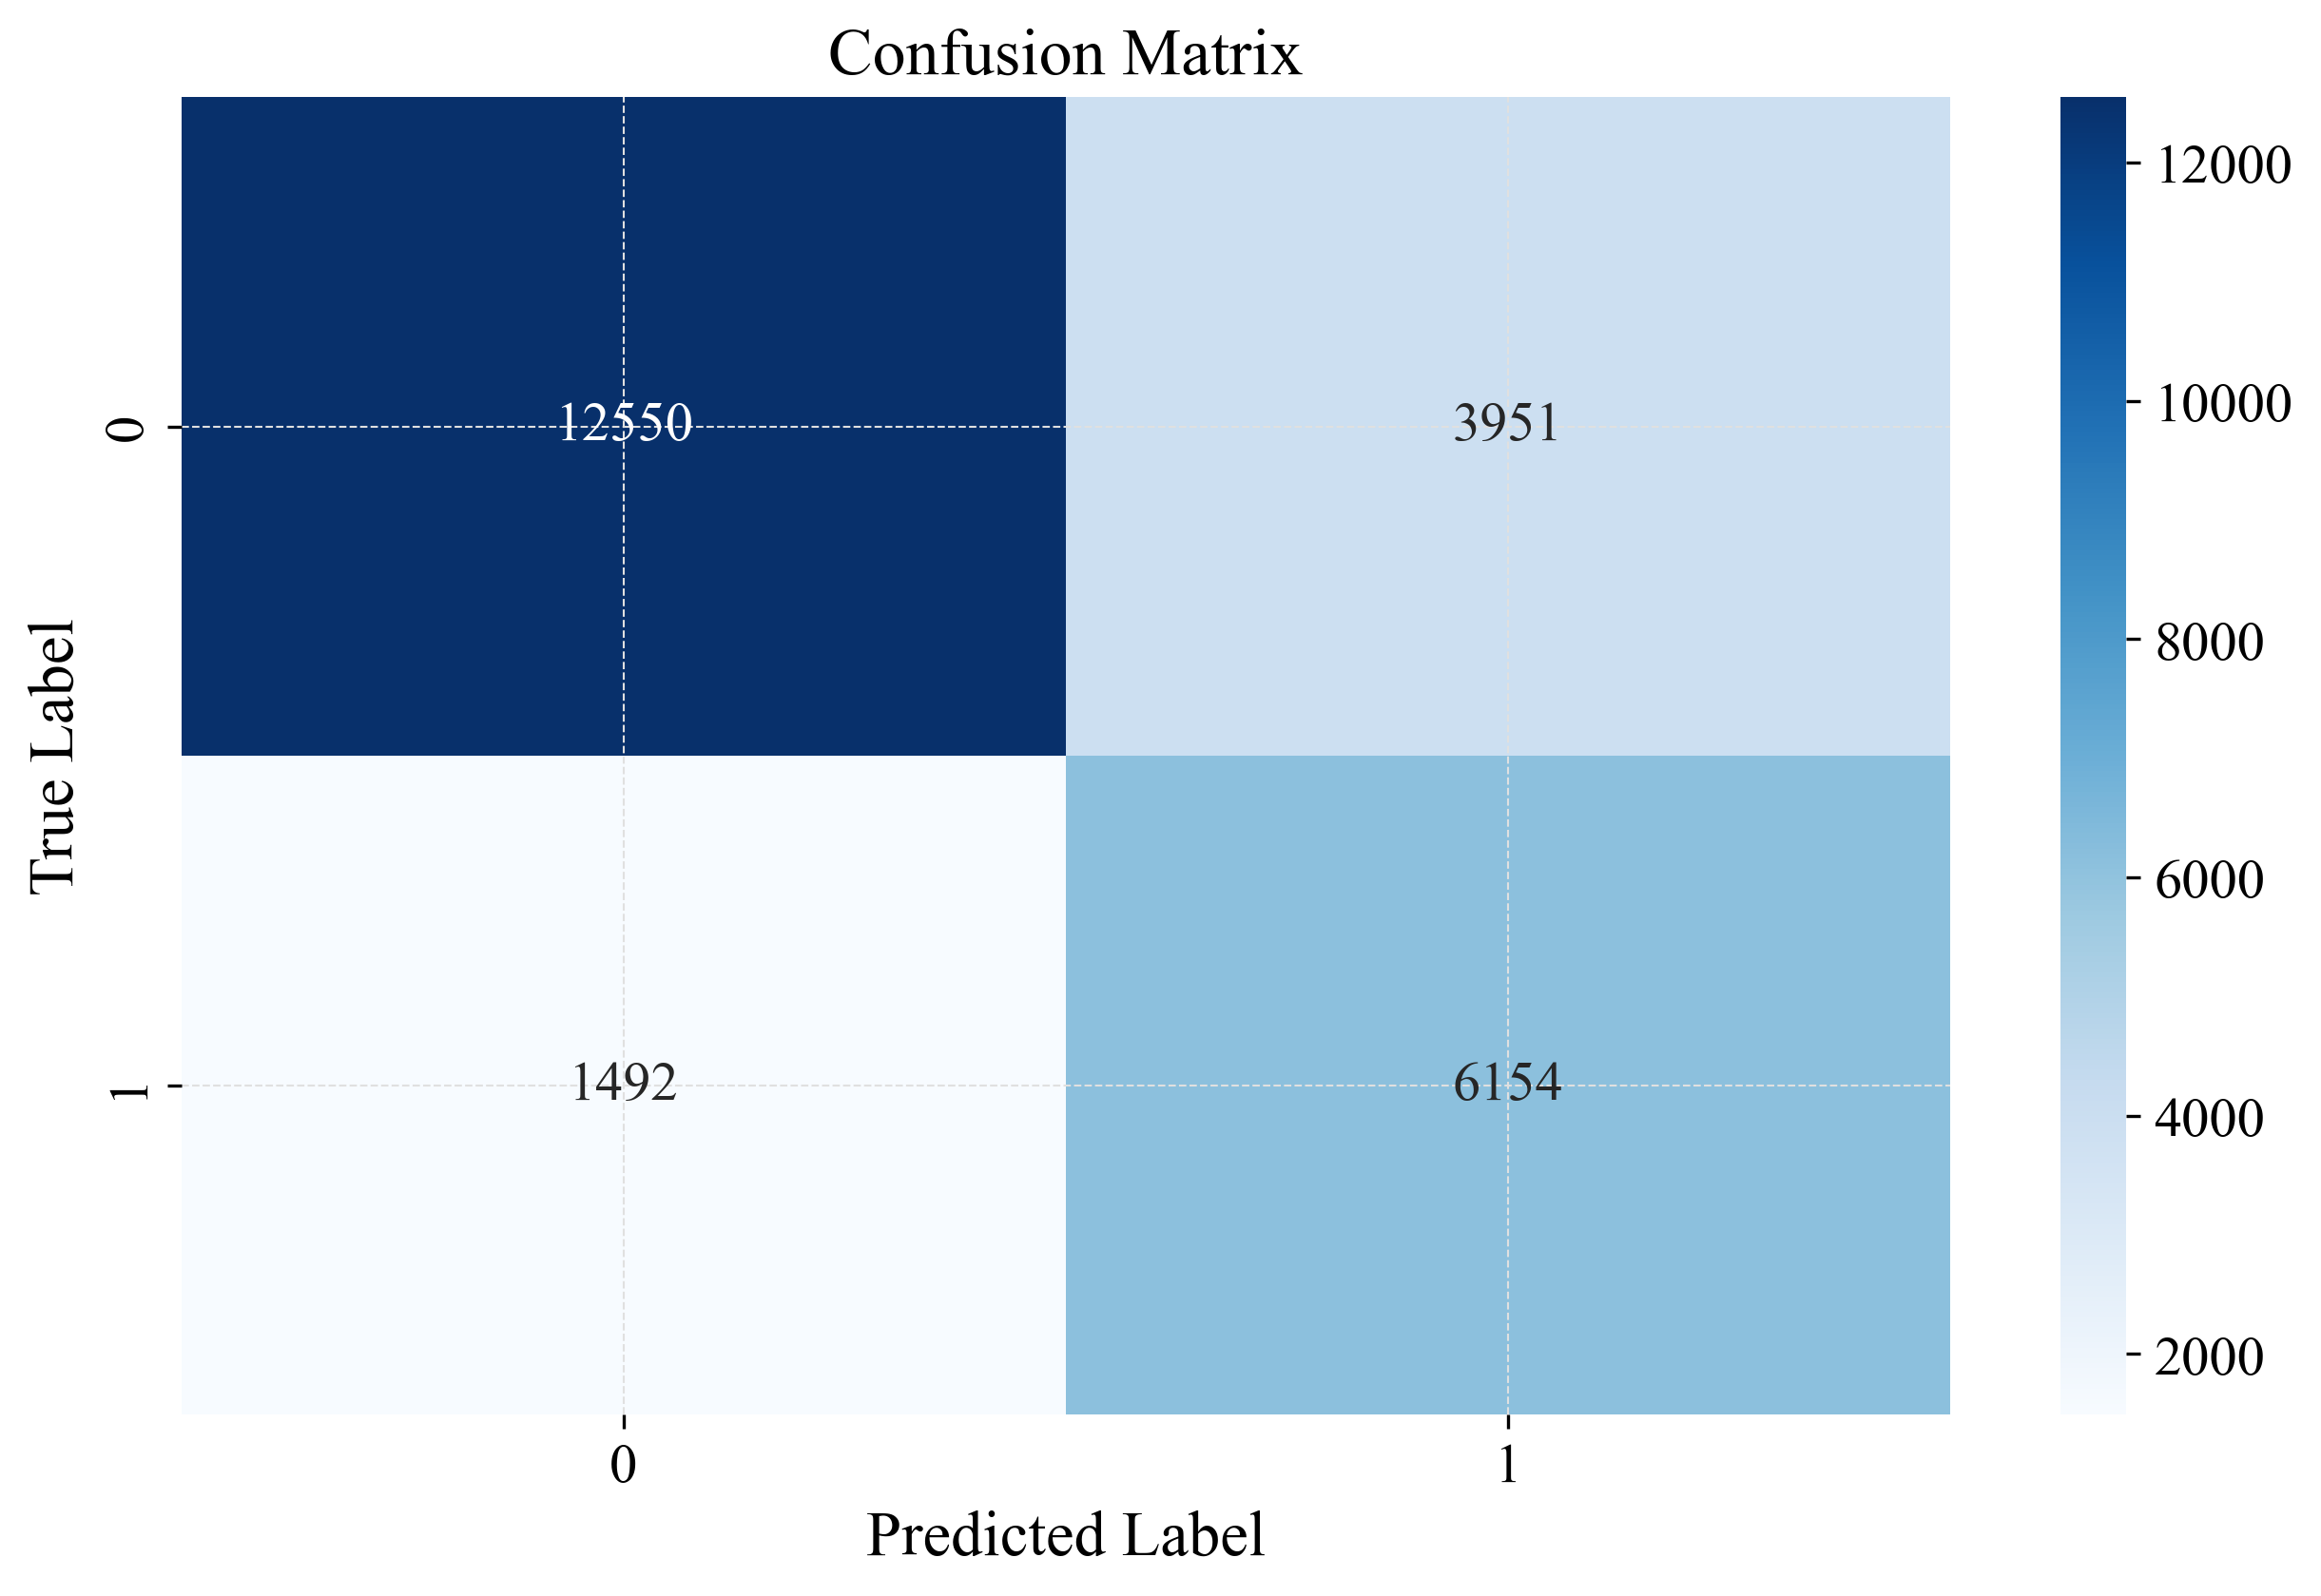
\includegraphics[width=0.8\textwidth]{figures/Figure33.png}
    \caption{Confusion Matrix for the Best Model}
    \label{fig:cha-4 figure2}
\end{figure}

\begin{figure}
    \centering
    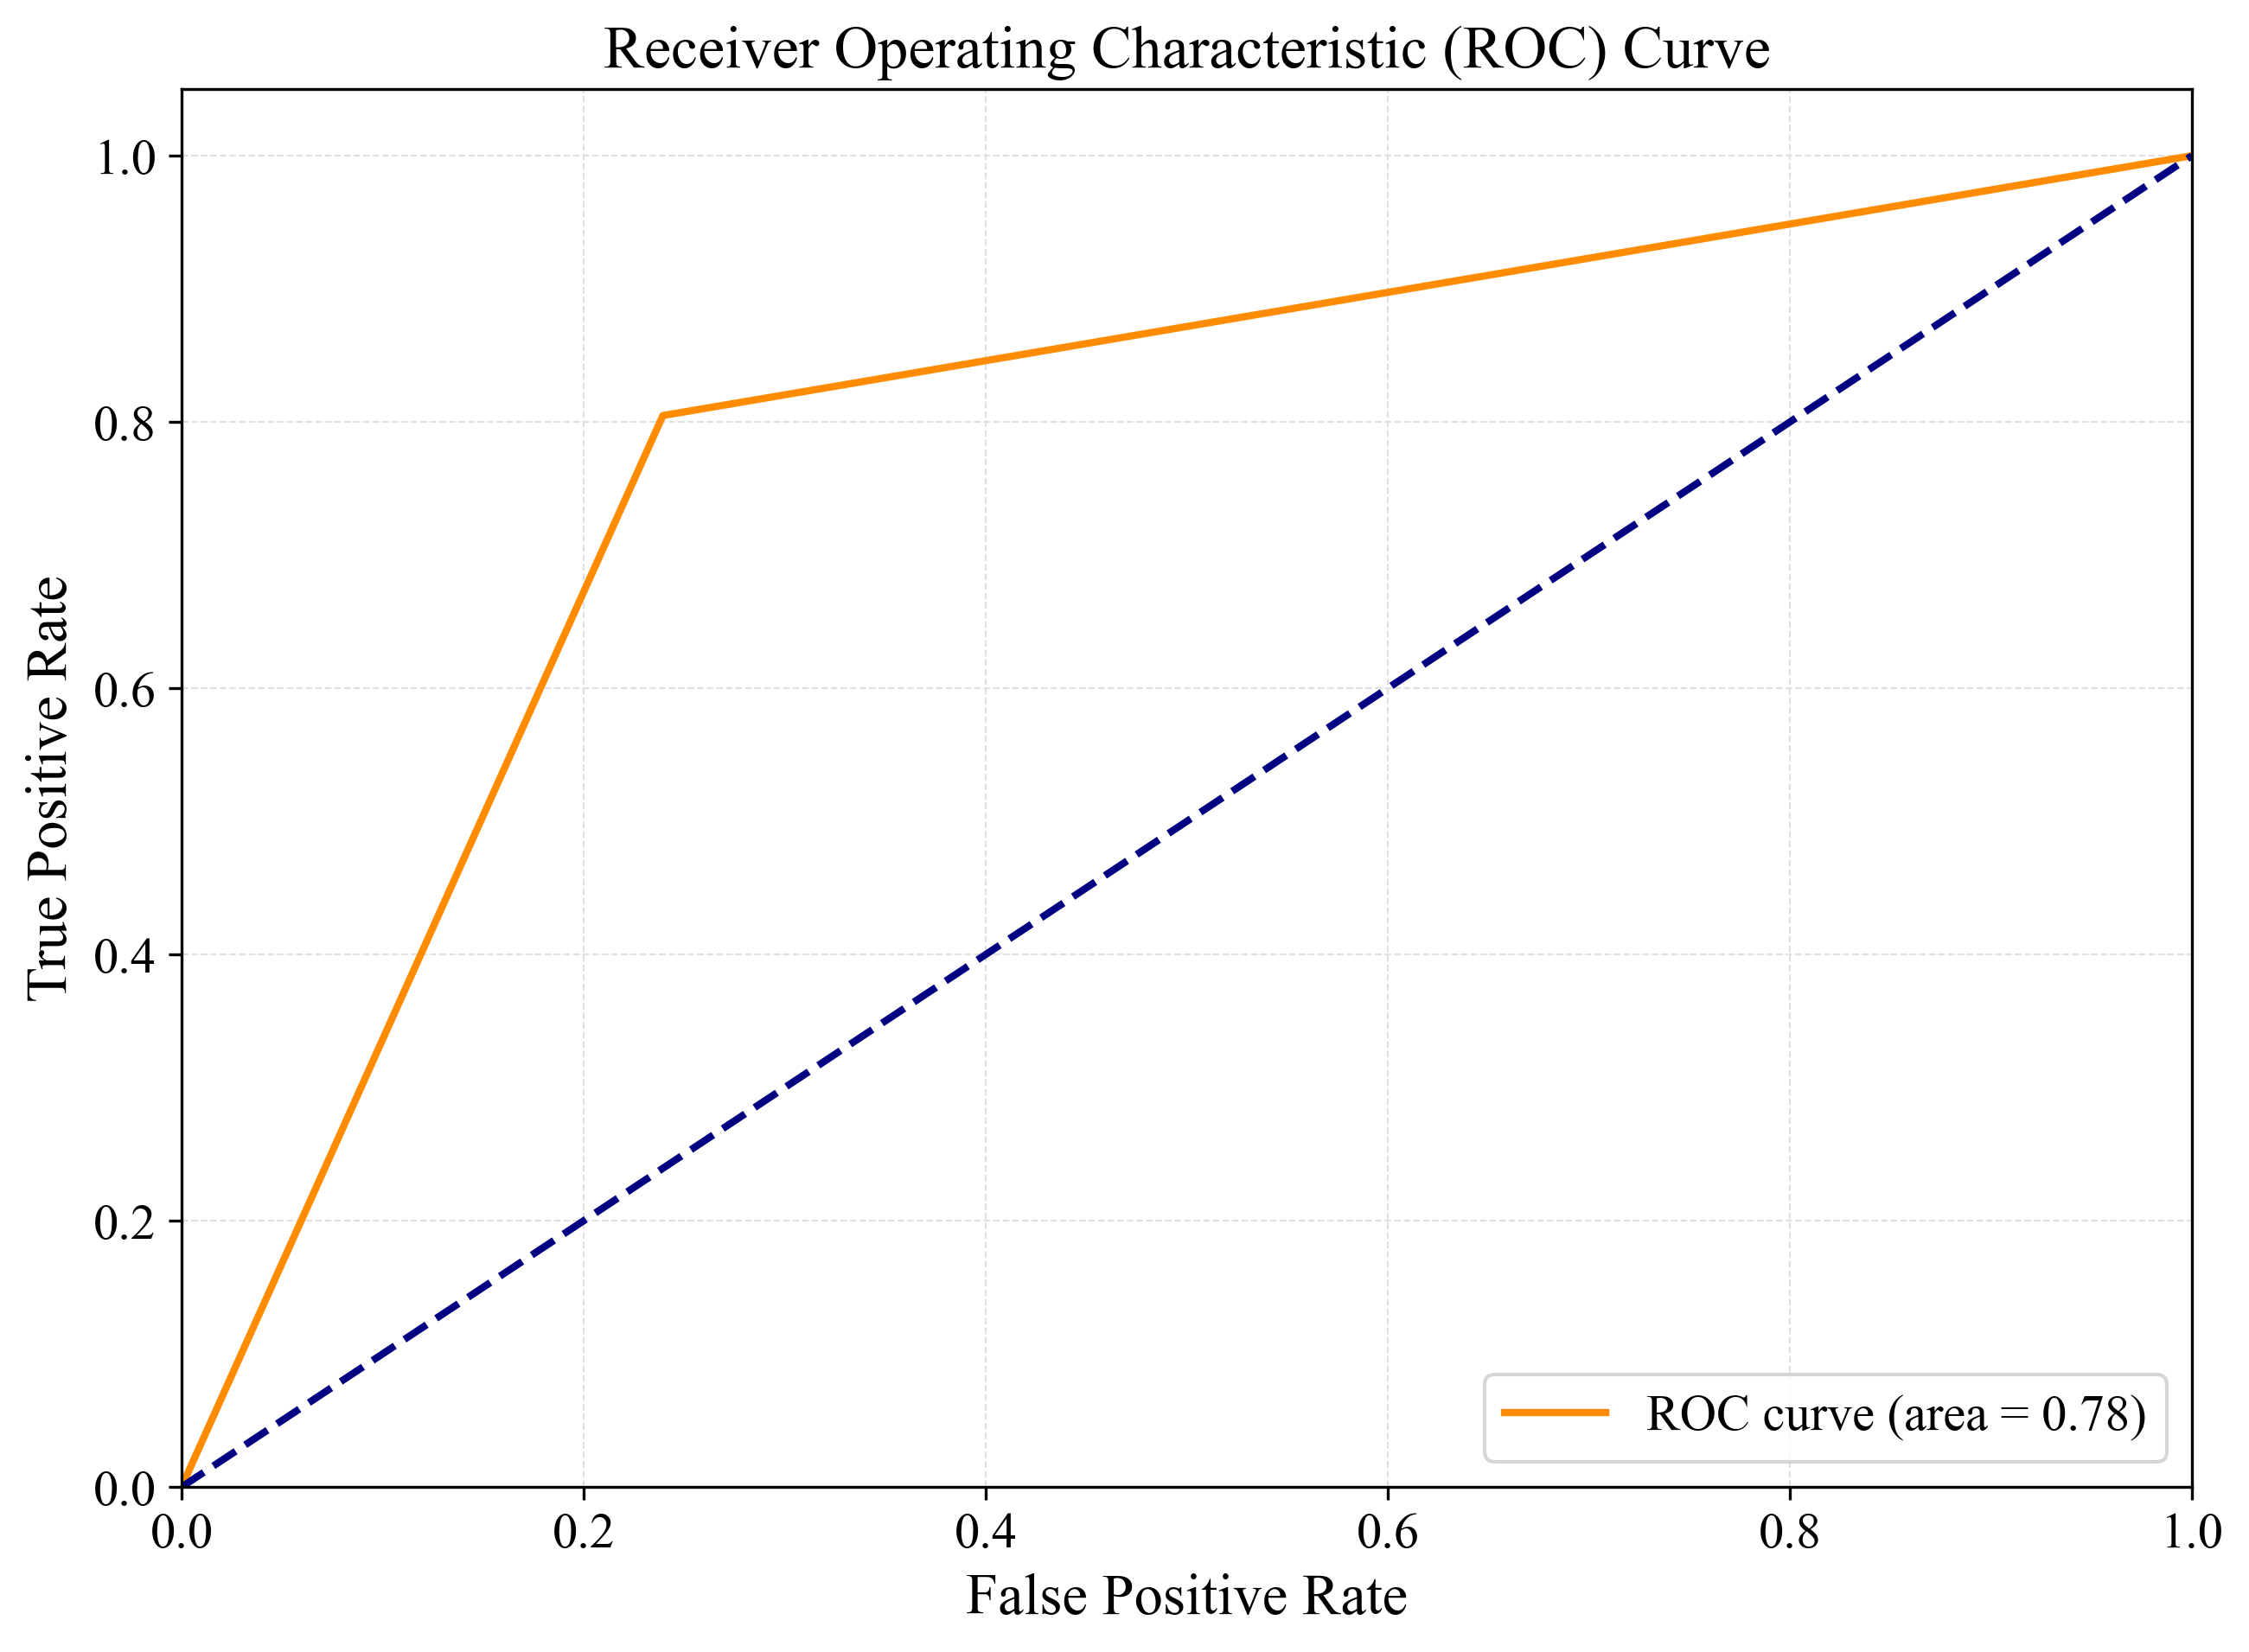
\includegraphics[width=0.8\textwidth]{figures/Figure34.png}
    \caption{ROC Curve for the Best Model}
    \label{fig:cha-4 figure3}
\end{figure}

\section{Future Steps}
\label{sec:chap4 section 3}

To further enhance the model's performance and prevent overfitting, several additional strategies can be considered (These are not implemented in the current model but can be explored in future iterations if time and resources permit):

\begin{itemize}
    \item \textbf{Data Augmentation:} Implementing advanced data augmentation techniques such as random rotations, translations, and horizontal flipping can help increase the diversity of the training data, making the model more robust.

    \item \textbf{Regularization:} Adding L2 regularization to the convolutional and dense layers can help prevent overfitting by penalizing large weights and encouraging simpler models.

    \item \textbf{Dropout Adjustment:} Experimenting with different dropout rates in the network can help determine the optimal level of regularization, ensuring that the model does not rely too heavily on any particular set of neurons.

    \item \textbf{Batch Normalization:} Integrating batch normalization layers can stabilize and accelerate the training process by normalizing the inputs to each layer, improving both training speed and model performance.

    \item \textbf{Learning Rate Scheduling:} Implementing advanced learning rate scheduling techniques such as cosine annealing or cyclic learning rates can help the model converge more efficiently and avoid local minima.

    \item \textbf{Ensemble Methods:} Training multiple models with different architectures and combining their predictions can lead to more robust and accurate results by leveraging the strengths of each model.

    \item \textbf{Transfer Learning:} Utilizing pre-trained models on similar datasets can provide a strong starting point, allowing the model to leverage learned features and improve performance with less training data.

    \item \textbf{Hyperparameter Tuning:} Conducting extensive hyperparameter tuning using techniques such as grid search or Bayesian optimization can help identify the optimal configuration for the model, leading to better performance.
\end{itemize}

% ------------------------------------------------------------------------------
% Reference list
% ------------------------------------------------------------------------------
\addcontentsline{toc}{chapter}{References}
\renewcommand\bibname{References}
\printbibliography

% ------------------------------------------------------------------------------
% Appendices
% ------------------------------------------------------------------------------
% --------------------------------------------------
% Appendices
% --------------------------------------------------
\appendix
\chapter{Code Snippets}
\label{app:appendix A}

\section{Image Preprocessing}
\label{app:app-A section1}

\begin{minted}{python}
# Define a function to read the DICOM images and resize them
def readAndReshapeDicomImages(data, image_size):
    patientIds = []
    labels = []
    images = []
    targets = []
    for i, row in notebook.tqdm(data.iterrows(), total=data.shape[0]):
        patientId = row["patientId"]
        label = row["class"]
        target = row["Target"]
        imagePath = row["path"]
        data_row_img = dcm.dcmread(imagePath)
        img = data_row_img.pixel_array
        # Convert the images to 3 channels as DICOM image pixel does not have color channels
        if len(img.shape) != 3 or (len(img.shape) == 3 and img.shape[2] != 3):
            img = np.stack((img,) * 3, -1)
        img = img - np.min(img)
        img = img / np.max(img)
        img = (img * 255).astype(np.uint8)
        img = cv2.resize(img, (image_size, image_size), interpolation=cv2.INTER_AREA)
        patientIds.append(patientId)
        labels.append(label)
        images.append(img)
        targets.append(target)
    return np.array(patientIds), np.array(labels), np.array(targets), np.array(images)
\end{minted}

\section{Model 1 Architecture}
\label{app:app-A section2}

\begin{minted}{python}
model1 = Sequential()

# Define the input shape
model1.add(Input(shape=(HEIGHT, WIDTH, NUM_CHANNELS)))

# First convolutional block
model1.add(Conv2D(filters=32, kernel_size=(5, 5), padding="Same", activation="relu"))
model1.add(Conv2D(filters=32, kernel_size=(5, 5), padding="Same", activation="relu"))
model1.add(MaxPooling2D(pool_size=(2, 2)))
model1.add(Dropout(0.2))

# Second convolutional block
model1.add(Conv2D(filters=64, kernel_size=(3, 3), padding="Same", activation="relu"))
model1.add(Conv2D(filters=64, kernel_size=(3, 3), padding="Same", activation="relu"))
model1.add(MaxPooling2D(pool_size=(2, 2), strides=(2, 2)))
model1.add(Dropout(0.3))

# Third convolutional block
model1.add(Conv2D(filters=128, kernel_size=(3, 3), padding="Same", activation="relu"))
model1.add(Conv2D(filters=128, kernel_size=(3, 3), padding="Same", activation="relu"))
model1.add(MaxPooling2D(pool_size=(2, 2), strides=(2, 2)))
model1.add(Dropout(0.4))

# Global Max Pooling
model1.add(GlobalMaxPooling2D())

# Fully connected layer
model1.add(Dense(256, activation="relu"))
model1.add(Dropout(0.5))

# Output layer
model1.add(Dense(NUM_CLASSES, activation="softmax"))

optimizer = RMSprop(learning_rate=0.001, rho=0.9, epsilon=1e-08)

# Compile model
model1.compile(
    optimizer=optimizer, loss="categorical_crossentropy", metrics=["accuracy"]
)

\end{minted}

\section{Model 2 Architecture}
\label{app:app-A section3}

\begin{minted}{python}
model2 = Sequential()

# Define the input shape
model2.add(Input(shape=(HEIGHT, WIDTH, NUM_CHANNELS)))

# First convolutional block
model2.add(Conv2D(filters=32, kernel_size=(5, 5), padding="Same", activation="relu"))
model2.add(Conv2D(filters=32, kernel_size=(5, 5), padding="Same", activation="relu"))
model2.add(MaxPooling2D(pool_size=(2, 2)))
model2.add(Dropout(0.2))

# Second convolutional block
model2.add(Conv2D(filters=64, kernel_size=(3, 3), padding="Same", activation="relu"))
model2.add(Conv2D(filters=64, kernel_size=(3, 3), padding="Same", activation="relu"))
model2.add(MaxPooling2D(pool_size=(2, 2), strides=(2, 2)))
model2.add(Dropout(0.3))

# Third convolutional block
model2.add(Conv2D(filters=128, kernel_size=(3, 3), padding="Same", activation="relu"))
model2.add(Conv2D(filters=128, kernel_size=(3, 3), padding="Same", activation="relu"))
model2.add(MaxPooling2D(pool_size=(2, 2), strides=(2, 2)))
model2.add(Dropout(0.4))

# Global Max Pooling
model2.add(GlobalMaxPooling2D())

# Fully connected layer
model2.add(Dense(256, activation="relu"))
model2.add(Dropout(0.5))

# Output layer
model2.add(Dense(NUM_CLASSES, activation="softmax"))

# Optimizer
optimizer2 = Adam(learning_rate=0.001, epsilon=1e-08, decay=0.0)

# Compile model
model2.compile(
    optimizer=optimizer2, loss="categorical_crossentropy", metrics=["accuracy"]
)
\end{minted}

\section{Model 3 Architecture}
\label{app:app-A section4}
\begin{minted}{python}
model3 = Sequential()
model3.add(Input(shape=(HEIGHT, WIDTH, NUM_CHANNELS)))
model3.add(Conv2D(filters=32, kernel_size=(3, 3), activation="relu"))
model3.add(MaxPooling2D(pool_size=(2, 2)))
model3.add(Dropout(0.25))
model3.add(Conv2D(filters=64, kernel_size=(3, 3), activation="relu"))
model3.add(MaxPooling2D(pool_size=(2, 2)))
model3.add(Dropout(0.25))
model3.add(GlobalMaxPooling2D())
model3.add(Dense(128, activation="relu"))
model3.add(Dropout(0.5))
model3.add(Dense(NUM_CLASSES, activation="softmax"))
model3.compile(optimizer="adam", loss="categorical_crossentropy", metrics=["accuracy"])
\end{minted}

\section{Fine tuning the model}
\label{app:app-A section5}

\begin{minted}{python}
lrr = ReduceLROnPlateau(
    monitor="val_accuracy", patience=10, verbose=1, factor=0.5, min_lr=0.00001
)
\end{minted}

\end{document}